\part{空间解析几何}
\section{向量代数}
空间解析几何中的向量是指一个三元数组$(a_1,a_2,a_3)$,习惯上表示为$\bm{a}=(a_1,a_2,a_3 )$或$\vec{a}=(a_1,a_2,a_3)$,
向量可以表示空间中的点和有项线段。

\begin{definition}
    设$\bm{a} = (a_1,a_2,a_3),\bm{b} = (b_1,b_2,b_3)$是向量,$\lambda$是实数,则有
    \begin{enumerate}[(1)]
        \item 加法:$\bm{a}+\bm{b} = (a_1+b_1,a_2+b_2,a_3+b_3)$
        \item 减法:$\bm{a}+\bm{b} = (a_1-b_1,a_2-b_2,a_3-b_3)$
        \item 数乘:$\lambda\bm{a} = \bm{a}\lambda = (\lambda a_1, \lambda a_2, \lambda a_3)$
        \item 内积:$\bm{a}\cdot\bm{b} = \bm{b}\cdots\bm{a} = a_1b_1+a_2b_2+a_3b_3$
        \item 外积:$\bm{a}\times\bm{b} = -\bm{b}\times\bm{a} = (a_2b_3-a_3b_2, a_3b_1-a_1b_3, a_1b_2-a_2b_1)$
        \item 三重积(混合积):$(\bm{a},\bm{b},\bm{c}) = (\bm{a}\times\bm{b})\cdot\bm{c}$
    \end{enumerate}
\end{definition}
其中内积满足交换性;外积满足\textcolor{red}{反}交换性;三重积满足轮换不变性和兑换反号性。
\subsection{线性运算}
在有关空间解析几何的题中,常常需要利用线性相关的等价表示,将条件转为另外一种条件,从而简化解题思路。
\begin{theorem}
    (三角形法则)
    \label{th:三角形法则}
    设$\bm{a},\bm{b},\bm{c}$为向量,则$\bm{a}+\bm{b}+\bm{c}=\bm{0}\iff$存在三点$A,B,C$,
    使得$\overrightarrow{AB}=\bm{c},\overrightarrow{BC}=\bm{a},\overrightarrow{CA}=\bm{b}$
\end{theorem}

\begin{definition}
    向量组$\bm{a}_1,\bm{a}_2,\cdots,\bm{a}_n$,如果\textcolor{red}{存在不全为零}的实数$\lambda_1,\lambda_2,\cdots,\lambda_n$,
    使得
    \[ \lambda_1\bm{a}_1 + \lambda_2\bm{a}_2 + \cdots + \lambda_n\bm{a}_n = \bm{0} \]
    则称向量$\bm{a}_1,\bm{a}_2,\cdots,\bm{a}_n$\textcolor{red}{\textbf{\textsf{线性相关}}}。

    换句话说,若
    \[ \lambda_1\bm{a}_1 + \lambda_2\bm{a}_2 + \cdots + \lambda_n\bm{a}_n = \bm{0} \]
    只有$0$解,即$\lambda_1 = \lambda_2 = \cdots = \lambda_n = 0$,则称\textcolor{red}{\textbf{\textsf{线性无关}}}。
\end{definition}

\begin{theorem}
    线性相关的一些等价性质。
    \begin{enumerate}[(1)]
        \item 设$\bm{a},\bm{b}$为向量,则$\bm{a},\bm{b}$线性相关
              $\iff \bm{a},\bm{b}$共线
              $\iff \dfrac{a_1}{b_1}=\dfrac{a_2}{b_2}=\dfrac{a_3}{b_3}$
              $\iff \bm{a}\times\bm{b}=0$
        \item 设$\bm{a},\bm{b},\bm{c}$为向量,则$\bm{a},\bm{b},\bm{c}$线性相关$\iff\bm{a},\bm{b},\bm{c}$共面$\iff(\bm{a},\bm{b},\bm{c})=0$
    \end{enumerate}
\end{theorem}
\pagebreak
\begin{marginfigure}
    \centering
    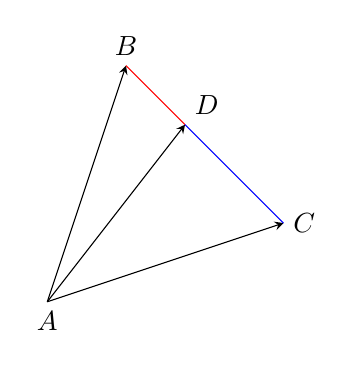
\begin{tikzpicture}
        \draw[-stealth] (0, 0) coordinate (A) -- (1, 3) coordinate (B);
        \draw[-stealth] (A) -- (3, 1) coordinate (C);
        \draw[-stealth] (A) -- (1.75, 2.25) coordinate (D);
        \draw[red] (B) -- (D);
        \draw[blue] (C) -- (D);

        \node [below] at (A) {$A$};
        \node [above] at (B) {$B$};
        \node [right] at (C) {$C$};
        \node [above right] at (D) {$D$};
    \end{tikzpicture}
    \caption{定比分点示意图,可以类比插值。}
\end{marginfigure}
\begin{theorem}
    (定比分点公式)
    若$D$点在$B$点与$C$点之间,向量$\overrightarrow{AD}$即可表达成向量$\overrightarrow{AB}$与向量$\overrightarrow{AC}$
    \[ \overrightarrow{AD} = \frac{|\overrightarrow{CD}|}{|\overrightarrow{BC}|}\overrightarrow{AB} + \frac{|\overrightarrow{BD}|}{|\overrightarrow{BC}|}\overrightarrow{AC} \]
    若$\dfrac{|\overrightarrow{CD}|}{|\overrightarrow{BC}|} = \lambda$,则有
    \[ \overrightarrow{AD} = \lambda\overrightarrow{AB} + (1-\lambda)\overrightarrow{AC} \]
\end{theorem}

\subsection{内积运算}
两个非$\bm{0}$向量$\bm{a},\bm{b}$的夹角定义为
\begin{equation}
    \langle\bm{a},\bm{b}\rangle = \arccos \frac{\bm{a}\cdot\bm{b}}{|\bm{a}||\bm{b}|}
\end{equation}
利用上式易得余弦公式
\begin{equation}
    \label{eq:余弦公式}
    |\bm{a}-\bm{b}|^2 = |\bm{a}|^2 + |\bm{b}|^2 - 2|\bm{a}||\bm{b}|\cos\langle\bm{a},\bm{b}\rangle
\end{equation}
同时易知两个相互垂直的向量$\bm{a},\bm{b}$有
\[ \bm{a}\perp\bm{b} \iff \bm{a}\cdot\bm{b} \]

向量$\bm{a}$在非$\bm{0}$向量$\bm{b}$上的投影为
\begin{equation}
    |\bm{a}|\cos\langle\bm{a},\bm{b}\rangle = \bm{a}\cdot\bm{b}_0 = \frac{\bm{a}\cdot\bm{b}}{|\bm{b}|}
\end{equation}
其中$\bm{b}_0$是$\bm{b}$的单位化向量。

由此可知,向量$\bm{a}$在$\bm{b}$上的投影向量可以表示为
\begin{equation}
    (\bm{a}\cdot\bm{b}_0)\bm{b}_0 = \frac{\bm{a}\cdot\bm{b}}{\bm{b}^2}\bm{b}
\end{equation}
于是$\bm{a}$关于$\bm{b}$的正交化向量为
\begin{equation}
    \bm{a} - \frac{\bm{a}\cdot\bm{b}}{\bm{b}^2}\bm{b}
\end{equation}

向量$\bm{a}$与坐标轴的夹角$\alpha,\beta,\gamma$称为方向角。方向角的计算可通过向量的单位化实现。
\begin{equation}
    \frac{\bm{a}}{|\bm{a}|} = (\cos\alpha,\cos\beta,\cos\gamma)
\end{equation}

\subsection{外积运算}
外积$\bm{a}\times\bm{b}$垂直与$\bm{a},\bm{b}$。同时其长度等于以$\bm{a},\bm{b}$为边的平行四边形面积。

外积还可以用行列式表示
\begin{equation}
    \bm{a}\times\bm{b} =
    \begin{vmatrix}
        \bm{i} & \bm{j} & \bm{k} \\
        a_1    & a_2    & a_3    \\
        b_1    & b_2    & b_3
    \end{vmatrix}
    =
    \left(
    \begin{vmatrix}
            a_2 & a_3 \\
            b_2 & b_3
        \end{vmatrix},
    \begin{vmatrix}
            a_3 & a_1 \\
            b_3 & b_1
        \end{vmatrix},
    \begin{vmatrix}
            a_1 & a_2 \\
            b_1 & b_2
        \end{vmatrix}
    \right)
\end{equation}

混合积可以表示为以$\bm{a},\bm{b},\bm{c}$所构成的平行六面体的体积。当构成右手系是为正数,左系为负数,线性相关时为$0$
\begin{equation}
    V = Sh = |\bm{a}\times\bm{b}||(\bm{e}\cdot\bm{c})| = |(\bm{a}\times\bm{b})\cdot\bm{c}| = |(\bm{a},\bm{b},\bm{c})|
\end{equation}
其中$\bm{e}$为底面的法向量。

混合积也可以用行列式表示
\begin{equation}
    (\bm{a},\bm{b},\bm{c}) = (\bm{a}\times\bm{b})\cdot\bm{c}
    =
    \begin{vmatrix}
        a_1 & a_2 & a_3 \\
        b_1 & b_2 & b_3 \\
        c_1 & c_2 & c_3 \\
    \end{vmatrix}
\end{equation}

设$\bm{a},\bm{b},\bm{c}$为向量,则有二叉积
\begin{eqnarray}
    \label{eq:二叉积}
    \bm{a}\times(\bm{b}\times\bm{c}) = (\bm{a}\cdot\bm{c})\bm{b} - (\bm{a}\cdot\bm{b})\bm{c}
\end{eqnarray}

若有线性表示
\[ \bm{x} = x_1\bm{a} + x_2\bm{b} + x_3\bm{c}, \quad \bm{y} = y_1\bm{a} + y_2\bm{b} + y_3\bm{c} \]
则有仿射叉积公式
\begin{equation}
    \bm{x}\times\bm{y}=
    \begin{vmatrix}
        \bm{b}\times\bm{c} & \bm{c}\times\bm{a} & \bm{a}\times\bm{b} \\
        x_1                & x_2                & x_3                \\
        y_1                & y_2                & y_3
    \end{vmatrix}
\end{equation}

\section{平面与直线}
\subsection{平面方程}
确定一个平面,常用的方法有
\begin{enumerate}[(1)]
    \item 不共线的三点唯一确定一个平面;
    \item 一直线和直线外的一点唯一确定一个平面;
    \item 两平行但不重合直线唯一确定一个平面;
    \item 两相交当不重合直线唯一确定一个平面;
    \item 给定一个点和一个法向量唯一确定一个平面;
    \item 给定一个点和两个不共线向量可以唯一确定一个平面,使该平面过给定点并与两个给定向量平行。
\end{enumerate}
\subsubsection{点法式方程}
设$\bm{r}_0=(x_0,y_0,z_0),\bm{n}=(A,B,C)$,则过$P(x_0,y_0,z_0)$点且与非$\bm{0}$向量$\bm{n}$垂直的平面方程为
\begin{equation}
    \label{eq:平面点法式方程}
    (\bm{r}-\bm{r}_0)\cdot \bm{n} = A(x-x_0) + B(y-y_0) + C(z-z_0) = 0
\end{equation}

\subsubsection{一般方程}
将\ref{eq:平面点法式方程}拆开可得平面一般方程。
\begin{equation}
    \label{eq:平面一般方程}
    Ax + By + Cz + D = 0
\end{equation}
向量$\bm{n}=(A,B,C)$为平面的法向量中的一个,当$A,B,C$确定时,则$D$唯一。坐标原点到平面的距离为
\begin{equation}
    d = \frac{|D|}{\sqrt{A^2+B^2+C^2}}
\end{equation}
\begin{proof}
    不妨设原点$O$到平面距离最短的点为$P(x_0,y_0,z_0)$,则向量$\overrightarrow{OP}$为平面的一个法向量,
    \[
        d
        = \frac{\left|\bm{n}\cdot\overrightarrow{OP}\right|}{|\bm{n}|}
        = \frac{|Ax_0 + By_0 + Cz_0|}{\sqrt{A^2+B^2+C^2}}
    \]
    同时点$P$在平面上,因此有
    \[ Ax_0 + By_0 + Cz_0 + D = 0 \]
    所以
    \[ d= \frac{|D|}{\sqrt{A^2+B^2+C^2}} \]
\end{proof}
显然两个平面一般方程中的$A,B,C$相同时,若$D$相同,则表示同一个平面,若$D$相反,则两平面关于原点对称。

\subsubsection{一点两向式}
如果$\bm{r}_1=(A_1,B_1,C_1),\bm{r}_2=(A_2,B_2,C_2)$式不共线向量,$\bm{r}_0=(x_0,y_0,z_0)$,
则过$P(x_0,y_0,z_0)$点且与$\bm{r}_1,\bm{r}_2$平行的平面的法向量为$\bm{r}_1\times\bm{r}_2$,因此平面方程为
\begin{equation}
    \label{eq:平面一点两向式}
    (\bm{r}-\bm{r}_0,\bm{r}_1,\bm{r}_2)=
    \begin{vmatrix}
        x-x_0 & y-y_0 & z-z_0 \\
        x_1   & y_1   & z_1   \\
        x_2   & y_2   & z_2
    \end{vmatrix}
    =0
\end{equation}

\subsubsection{参数方程}
根据平面方程\ref{eq:平面一点两向式},有
\begin{equation}
    \label{eq:平面参数方程}
    \bm{r} = \bm{r}_0 + t_1\bm{r}_1 + t_2\bm{r}_2
\end{equation}
或
\begin{equation}
    \begin{cases}
        x = x_0 + t_1 A_1 + t_2A_2, \\
        y = y_0 + t_1 B_1 + t_2B_2, \\
        z = z_0 + t_1 C_1 + t_2C_2.
    \end{cases}
\end{equation}

\subsubsection{三点式方程}
设$A(x_1,y_1,z_1),B(x_2,y_2,z_2),C(x_3,y_3,z_3)$为不共线三点,则过$A,B,C$三点的平面方程为
\begin{equation}
    \label{eq:平面三点式方程}
    (\bm{r}-\bm{r}_1,\bm{r}_2-\bm{r}_1, \bm{r}_3-\bm{r}_1)
    =
    \begin{vmatrix}
        x-x_1   & y-y_1   & z-z_1   \\
        x_2-x_1 & y_2-y_1 & z_2-z_1 \\
        x_3-x_1 & y_3-y_1 & z_3-z_1 \\
    \end{vmatrix}
    =0
\end{equation}

\subsubsection{截距式方程}
如果平面交$x$轴,$y$轴,$z$轴于点$A(a,0,0),B(0,b,0),C(0,0,c)$且$abc\neq 0$时,将三点带入\ref{eq:平面三点式方程}则方程为
\begin{equation}
    \label{eq:平面截距式方程}
    \frac{x}{a} + \frac{y}{b} + \frac{z}{c} = 1
\end{equation}
向量$(a,b,c)$为平面的一个法向量。

\subsubsection{两点一向式}
设$A(x_1,y_1,z_1),B(x_2,y_2,z_2)$是空间的两个点,$\bm{v}$是不平行于$\overrightarrow{AB}$的一个向量,
则过点$A,B$且平行于$\bm{v}=(v_1,v_2,v_3)$的平面方程为
\begin{equation}
    \label{eq:平面两点一向式}
    (\bm{r}-\bm{r}_1,\bm{r}_2-\bm{r}_1,\bm{v}) =
    \begin{vmatrix}
        x-x_1   & y-y_1   & z-z_1   \\
        x_2-x_1 & y_2-y_1 & z_2-z_1 \\
        v_1     & v_2     & v_3
    \end{vmatrix}
    =0
\end{equation}

\subsubsection{法式方程}
如果平面于原点的距离为$p$且法向量$\bm{n}_0=(\cos\alpha,\cos\beta,\cos\gamma)$,则该平面方程为
\begin{equation}
    \label{eq:平面法式方程}
    \bm{r}\cdot\bm{n}_0 = x\cos\alpha + y\cos\beta + z\cos\gamma = p
\end{equation}

\subsection{直线方程}
建立直线方程,常用的我方法有:
\begin{enumerate}[(1)]
    \item 两个不同点唯一确定一条直线;
    \item 过一个点且于已知直线平行的直线唯一确定一条直线;
    \item 两个相交但不重合平面唯一确定一条直线。
\end{enumerate}

\subsubsection{参数方程}
设$\bm{r}_0=(x_0,y_0,z_0),\bm{v}=(v_1,v_2,v_3)$,则过$P(x_0,y_0,z_0)$且与向量$\bm{v}$平行的直线方程为
\begin{equation}
    \label{eq:直线参数方程}
    \bm{r}-\bm{r}_0 = t\bm{v}\text{ 或~} \bm{r} = \bm{r}_0 + t\bm{v}
\end{equation}

\subsubsection{点向式方程}
在直线方程\ref{eq:直线参数方程}中消去参数$t$可得点向式方程
\begin{equation}
    \label{eq:直线点向式方程}
    \frac{x-x_0}{v_1} = \frac{y-y_0}{v_2} = \frac{z-z_0}{v_3}
\end{equation}
其中$v_1,v_2,v_3$允许有一个或两个为$0$,例如当$v_3=0$时,原方程应理解为
\[
    \begin{cases}
        \frac{x-x_0}{v_1} = \frac{y-y_0}{v_2}, \\
        z=z_0.
    \end{cases}
\]

\subsubsection{交面式方程}
直线可以看成是两平面的交线,交线方向可以用法向量的叉积确定,可简记为“\textbf{\textsf{交线方向用叉积}}”

设$\pi_1 : A_1x + B_1y + C_1z + D_1 = 0,\, \pi_2 : A_2x + B_2y + C_2z + D_2 = 0$是两个相交于一条直线的平面方程,
则交线方程为
\begin{equation}
    \label{eq:直线交面式方程}
    L:\begin{cases}
        A_1x + B_1y + C_1z + D_1 = 0, \\
        A_2x + B_2y + C_2z + D_2 = 0.
    \end{cases}
\end{equation}
其直线的方向向量为
\[
    \bm{v} = \bm{n}_1\times\bm{n}_2 =
    \left(
    \begin{vmatrix}
            B_1 & C_1 \\
            B_2 & C_2
        \end{vmatrix},
    \begin{vmatrix}
            C_1 & A_1 \\
            C_2 & A_2
        \end{vmatrix},
    \begin{vmatrix}
            A_1 & B_1 \\
            A_2 & B_2
        \end{vmatrix}
    \right)
\]

\subsubsection{两点式方程}
设$\bm{r}_1=(x_1,y_1,z_1),\bm{r}_2=(x_2,y_2,z_2)$,则过$A(x_1,y_1,z_1),B(x_2,y_2,z_2)$两点的直线方程为
\begin{equation}
    \bm{r}-\bm{r}_1 = t(\bm{r}_2-\bm{r}_1)
\end{equation}
或
\begin{equation}
    \label{eq:直线两点式方程}
    \frac{x-x_1}{x_2-x_1} = \frac{y-y_1}{y_2-y_1} = \frac{z-z_1}{z_2-z_1}
\end{equation}

\subsubsection{过直线的平面系}
设直线
\[
    L: \begin{cases}
        A_1x+B_1y+C_1z+D_1 = 0, \\
        A_2x+B_2y+C_2z+D_2 = 0。 \\
    \end{cases}
\]
则过该直线的所有平面满足
\begin{equation}
    \pi :  (\lambda A_1 + \eta A_1)x + (\lambda A_2 + \eta A_2)y + (\lambda A_3 + \eta A_3)z + (\lambda A_1 + \eta A_1)=0
\end{equation}
其中$\lambda,\eta$为构成直线的两个平面的线性组合系数。所得平面系得法向量则为两个平面的法向量的线性组合。
一般可令$\lambda=1$或$\eta=1$使得该平面系方程只有一个系数变量。通过求解约束条件方程得出该系数变量的值。

\subsection{点线面关系}
\subsubsection{线线关系}
设
\begin{align*}
    L_1 : \frac{x-x_1}{u_1} = \frac{y-y_1}{u_2} = \frac{z-z_1}{u_3}, \\
    L_2 : \frac{x-x_2}{v_1} = \frac{y-y_2}{v_2} = \frac{z-z_2}{v_3}
\end{align*}
为两直线$L_1,L_2$方程,方向向量分别为
\[ \bm{u}=(u_1,u_2,u_3)\,\quad\bm{v}=(v_1,v_2,v_31) \]
则向量$\bm{u},\bm{v}$的夹角就是直线$L_1,L_2$的夹角。即
\[
    \cos\theta
    = \frac{\bm{u}\cdot\bm{v}}{|\bm{u}||\bm{v}|}
    = \frac{u_1v_1 + u_2v_2 + u_3v_3}{\sqrt{u_1^2+u_2^2+u_3^2}\sqrt{v_1^2+v_2^2+v_3^2}}
\]

特别有,两直线的垂直条件:
\[ L_1 \perp L_2 \iff \bm{u}\cdot\bm{v} = u_1v_1 + u_2v_2 + u_3v_3 = 0 \]
两直线平行条件:
\[ L_1 \parallel L_2 \iff \bm{u}\times\bm{v} = \bm{0} \iff \frac{u_1}{v_1} = \frac{u_2}{v_2} = \frac{u_3}{v_v}  \]

\subsubsection{线面关系}
设
\begin{align*}
    L   & : \frac{x-x_1}{v_1} = \frac{y-y_1}{v_2} = \frac{z-z_1}{v_3} \\
    \pi & : Ax+By+Cz+D=0
\end{align*}
则直线$L$方向向量为$\bm{v}=(v_1,v_2,v_3)$,平面$\pi$的法向量为$\bm{n}=(A,B,C)$,
则直线$L$与平面$\pi$平行的条件为
\[ \bm{v}\cdot\bm{n} = Av_1 + Bv_2 + Cv_3 = 0 \]
相交条件为
\[ \bm{v}\cdot\bm{n} = Av_1 + Bv_2 + Cv_3 \neq 0 \]

将直线写成参数形式
\[
    \begin{cases}
        x = x_0 + v_1t \\
        y = y_0 + v_2t \\
        z = z_0 + v_3t
    \end{cases}
\]
带入平面方程中可得
\[ A(x_0 + v_1t)+B(y_0 + v_2t)+C(z_0 + v_3t)+D=0 \]
解得
\[ t = -\frac{Ax_0+By_0+Cz_0+D}{Av_1 + Bv_2 + Cv_3} \]
将此值带入直线参数方程可得交点坐标。

直线$L$与平面$\pi$的夹角为$\theta = \dfrac{\pi}{2} - \langle\bm{v},\bm{n}\rangle$因此有
\[
    \sin\theta = \cos\left(\frac{\pi}{2}-\theta\right)
    = \frac{|\bm{v}\cdot\bm{n}|}{|\bm{v}||\bm{n}|}
    = \frac{|Av_1 + Bv_2 + Cv_3|}{\sqrt{A^2+B^2+C^2}\sqrt{v_1^2+v_2^2+v_3^2}}
\]

\subsubsection{两平面关系}
两平面之间要么重合,要么不等平行,要么交于一直线。设
\[
    \begin{cases}
        \pi_1 : A_1x+B_1y+C_1z+D_1=0 \\
        \pi_2 : A_2x+B_2y+C_2z+D_2=0
    \end{cases}
\]
是两个平面方程,且法向量为$\bm{n}_1=(A_1,B_1,C_1),\bm{n}_2=(A_2,B_2,C_2)$,则有
\begin{align*}
    \pi_1 = \pi_2                           & \iff \frac{A_1}{A_2} = \frac{B_1}{B_2} = \frac{C_1}{C_2} = \frac{D_1}{D_2},    \\
    \pi_1 \parallel \pi_2, \pi_1 \neq \pi_2 & \iff \frac{A_1}{A_2} = \frac{B_1}{B_2} = \frac{C_1}{C_2} \neq \frac{D_1}{D_2}, \\
    \pi_1 \parallel \pi_2                   & \iff \bm{n}_1 \parallel \bm{n}_2,                                              \\
    \pi_1 \perp \pi_2                       & \iff \bm{n}_1 \perp \bm{n}_2,                                                  \\
    \langle\pi_1,\pi_2\rangle               & = \langle\bm{n}_1,\bm{n}_2\rangle.
\end{align*}
特别需要记住,\textbf{\textsf{两平面夹角就是两法线夹角}}。由此可知,如果$ABCD$是平面$\pi_1$上的平行四边形,
$A'B'C'D'$是四边形$ABCD$在平面$\pi_2$上的投影,则有\textcolor{red}{\textbf{\textsf{面积投影公式}}}:
\[
    \left\lvert \overrightarrow{A'B'}\times\overrightarrow{A'D'}\right\rvert = \left\lvert \overrightarrow{AB}\times\overrightarrow{AD}\right\rvert\cos\langle\bm{n}_1,\bm{n}_2\rangle
\]
更一般地,如果$S_\text{原}$是平面$\pi_1$上的某图形面积,$S_\text{投}$是该图形在平面$\pi_2$上的投影面积,则有
\begin{equation}
    \label{eq:面积投影公式}
    S_\text{原}  = S_\text{投}\cos\langle\bm{n}_1,\bm{n}_2\rangle
\end{equation}

\subsubsection{三平面关系}
\textcolor{red}{无重合}三平面的位置关系可分,
\textcolor{red}{\textbf{\textsf{三面平行}}},
\textcolor{red}{\textbf{\textsf{两平一斜}}},
\textcolor{red}{\textbf{\textsf{唯一交点}}},
\textcolor{red}{\textbf{\textsf{唯一交线}}},
\textcolor{red}{\textbf{\textsf{不平不交}}}五种情况。

设无重合三平面方程为
\[
    \begin{cases}
        \pi_1 : A_1x+B_1y+C_1z+D_1=0 \\
        \pi_2 : A_2x+B_2y+C_2z+D_2=0 \\
        \pi_3 : A_3x+B_3y+C_3z+D_3=0
    \end{cases}
\]
其中$\bm{n}_1=(A_1,B_1,C_1),\bm{n}_2=(A_2,B_2,C_2),\bm{n}_3=(A_3,B_3,C_3)$分别是$\pi_1,\pi_2,\pi_3$的法向量。
则有
\begin{enumerate}[(1)]
    \item 三面平行 $\iff \bm{n}_1\parallel\bm{n}_2\parallel\bm{n}_3$;
    \item 两平一斜 $\iff \bm{n}_i\parallel\bm{n}_j\nparallel\bm{n}_k,\,\{i,j,k\}=\{1,2,3\}$;
    \item 唯一交点 $\iff (\bm{n}_1,\bm{n}_2,\bm{n}_3) \neq 0$;
    \item 唯一交线 $\iff (\bm{n}_1,\bm{n}_2,\bm{n}_3)=0$且三面有交;
    \item 不平不交 $\iff$ 三面无交且$\bm{n}_1,\bm{n}_2,\bm{n}_3$两两线性无关。
\end{enumerate}
\begin{figure}[htbp]
    \centering
    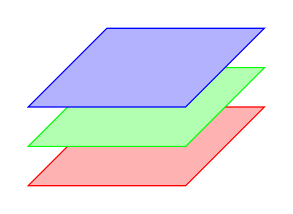
\begin{tikzpicture}
        \draw[color=red,fill=red!30] (0,0) -- (1,1) -- (3,1) -- (2,0) -- cycle;
        \draw[color=green,fill=green!30] (0,0.5) -- (1,1.5) -- (3,1.5) -- (2,0.5) -- cycle;
        \draw[color=blue,fill=blue!30] (0,1) -- (1,2) -- (3,2) -- (2,1) -- cycle;
    \end{tikzpicture}
    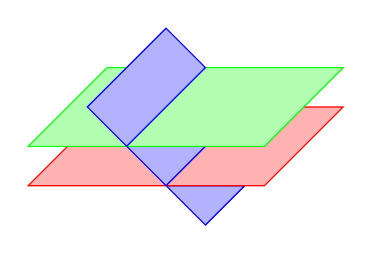
\begin{tikzpicture}
        \draw[color=blue,fill=blue!30] (1.75,0) -- (2.25,-0.5) -- (2.75,0) -- cycle;
        \draw[color=red,fill=red!30] (0,0) -- (3,0) -- (4,1) -- (1,1) -- cycle;
        \draw[color=blue,fill=blue!30] (1.25,0.5) -- (1.75,0) -- (2.25,0.5) -- cycle;
        \draw[color=green,fill=green!30] (0,0.5) -- (1,1.5) -- (4,1.5) -- (3,0.5) -- cycle;
        \draw[color=blue,fill=blue!30] (1.25,0.5) -- (2.25,1.5) -- (1.75,2) -- (0.75,1) -- cycle;
    \end{tikzpicture}
    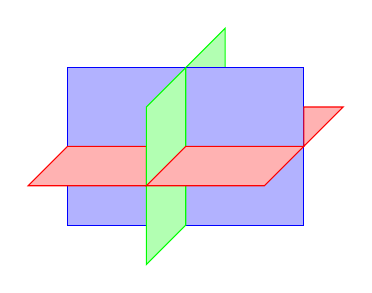
\begin{tikzpicture}
        \draw[color=green,fill=green!30] (1.5,2) -- (2,2.5) -- (2,2) -- cycle;
        \draw[color=blue,fill=blue!30] (0,0) -- (0,2) -- (3,2) -- (3,0) -- cycle;
        \draw[color=red,fill=red!30] (3,1) -- (3.5,1.5) -- (3,1.5) -- cycle;
        \draw[color=red,fill=red!30] (-0.5,0.5) -- (1,0.5) -- (1,1) -- (0,1) -- cycle;
        \draw[color=green,fill=green!30] (1.5,2) -- (1,1.5) -- (1,-0.5) -- (1.5,0) -- cycle;
        \draw[color=red,fill=red!30] (1,0.5) -- (2.5,0.5) -- (3,1) -- (1.5,1) -- cycle;
    \end{tikzpicture}
    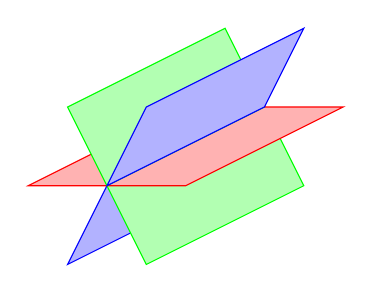
\begin{tikzpicture}
        \draw[color=blue,fill=blue!30] (1,0) -- (0.5,-1) -- (2.5,0) -- (3,1) -- cycle;
        \draw[color=green,fill=green!30] (1,0) -- (1.5,-1) -- (3.5,0) -- (3,1) -- cycle;
        \draw[color=red,fill=red!30] (0,0) -- (2,0) -- (4,1) -- (2,1) -- cycle;
        \draw[color=green,fill=green!30] (1,0) -- (0.5,1) -- (2.5,2) -- (3,1) -- cycle;
        \draw[color=blue,fill=blue!30] (1,0) -- (1.5,1) -- (3.5,2) -- (3,1) -- cycle;
    \end{tikzpicture}
    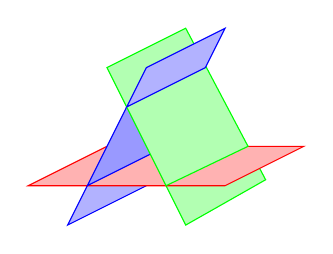
\begin{tikzpicture}
        \draw[color=blue,fill=blue!30] (0.5,-0.5) -- (1.5,0) -- (1.75,0.5) -- (0.75,0) -- cycle;
        \draw[color=green,fill=green!30] (1.75,0) -- (2.7913043055990334,0.5) -- (3.0151685536285298,0.07564192477122947) -- (2,-0.5) -- cycle;
        \draw[color=red,fill=red!30] (0,0) -- (1,0.5) -- (3.5,0.5) -- (2.5,0) -- cycle;
        \draw[color=blue,fill=blue!40] (0.75,0) -- (1.75,0.5) -- (2.25,1.5) -- (1.25,1) -- cycle;
        \draw[color=green,fill=green!30] (1,1.5) -- (1.75,0) -- (2.7913043055990334,0.5) -- (2,2) -- cycle;
        \draw[color=blue,fill=blue!30] (1.25,1) -- (2.25,1.5) -- (2.5,2) -- (1.5,1.5) -- cycle;
    \end{tikzpicture}
    \caption{五种不重合三平面关系}
\end{figure}

\subsubsection{点到平面的距离}
设$Ax+By+Cz+D=0$是一个平面,$\bm{n}=(A,B,C)$为其法向量,$P=(x_0,y_0,z_0)$为平面外一点,任取平面上一点$M(x,y,z)$,则点$P$到平面的距离为
\begin{equation}
    \label{eq:点到平面的距离公式}
    d = \left\lvert \overrightarrow{PM}\cdot\frac{\bm{n}}{|\bm{n}|}\right\rvert
    = \frac{|A(x-x_0) + B(y-y_0) + C(z-z_0)|}{\sqrt{A^2+B^2+C^2}}
    = \frac{|Ax_0+By_0+Cz_0+D|}{\sqrt{A^2+B^2+C^2}}
\end{equation}

\subsubsection{点到直线的距离}
设$\dfrac{x-x_0}{v_1} = \dfrac{y-y_0}{v_2} = \dfrac{z-z_0}{v_3}$是一条直线,$\bm{v}=(v_1,v_2,v_3)$,
点$P(x_1,y_1,z_1)$是直线外一点,$M$点坐标为$(x_0,y_0,z_0)$,利用平行四边形的面积可推出所求距离$d$为
\begin{marginfigure}
    \centering
    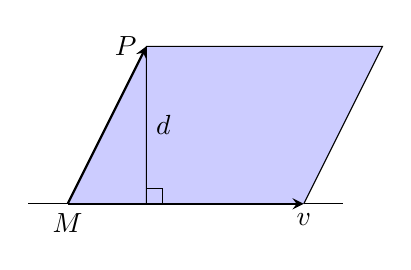
\begin{tikzpicture}
        \draw (-0.5, 0) -- (3.5, 0);
        \coordinate (M) at (0, 0);
        \coordinate (L) at (3, 0);
        \coordinate (P) at (1, 2);
        \coordinate (D) at (4, 2);
        \fill[blue!20!white] (M) -- (L) -- (D) -- (P) -- cycle;
        \draw[-stealth, thick] (M) -- (L);
        \draw[-stealth, thick] (M) -- (P);
        \draw (L) -- (4, 2)  -- (P) -- (1, 0) node [pos=0.5,right] {$d$};
        \draw (1.2, 0) rectangle (1, 0.2);
        \node[below] at (M) {$M$};
        \node[below] at (L) {$\bm{v}$};
        \node[left] at (P) {$P$};
    \end{tikzpicture}
    \caption{点到直线的距离示意图}
\end{marginfigure}
\begin{equation}
    \label{eq:点到直线的距离公式}
    d = \frac{\left\lvert \overrightarrow{PM}\times\bm{v}\right\rvert}{|\bm{v}|}
\end{equation}

\subsubsection{异面直线间的距离}
设$L_1 : \bm{r} = \bm{r}_1 + t\bm{u},\, L_2 : \bm{r} = \bm{r}_2 + t\bm{v}$是两条异面直线,
则公垂线长度为
\begin{equation}
    \label{eq:异面直线间的距离公式}
    d
    = \left\lvert (\bm{r}_2 - \bm{r}_1)\cdot \frac{\bm{u}\times\bm{v}}{|\bm{u}\times\bm{v}|} \right\rvert
    = \frac{|(\bm{r}_2 - \bm{r}_1, \bm{u}, \bm{v})|}{|\bm{u}\times\bm{v}|}
\end{equation}
\begin{marginfigure}
    \centering
    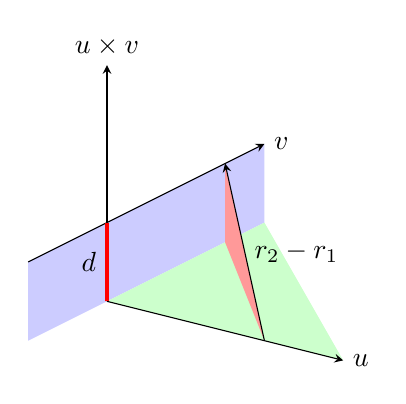
\begin{tikzpicture}
        \coordinate (0) at (0, 0);
        \coordinate (1) at (0, 3);
        \coordinate (2) at (-1, 0.5);
        \coordinate (3) at (2, 2);
        \coordinate (4) at (3, -0.75);
        \coordinate (5) at (1.5, 1.75);
        \coordinate (6) at (2, -0.5);
        \coordinate (7) at (-1, -0.5);
        \coordinate (8) at (2, 1);
        \coordinate (9) at (1.5, 0.75);
        \coordinate (10) at (0, 1);
        \fill[blue!20!white] (7) -- (8) -- (3) -- (2) -- cycle;
        \fill[green!20!white] (0) -- (8) -- (4) --  cycle;
        \fill[red!40!white] (6) -- (5) -- (9) --  cycle;
        \draw[-stealth] (2) -- (3) node[right] {$\bm{v}$};
        \draw[-stealth] (0) -- (1) node[above] {$\bm{u}\times\bm{v}$};
        \draw[-stealth] (0) -- (4) node[right] {$\bm{u}$};
        \draw[-stealth] (6) -- (5) node[pos=0.5,right] {$\bm{r}_2-\bm{r}_1$};
        \draw[red,very thick] (0) -- (10) node[pos=0.5, left, black] {$d$};
    \end{tikzpicture}
    \caption{异面直线间的距离示意图}
\end{marginfigure}

\section{曲线与曲面}
\subsection{空间曲面}
\subsubsection{曲面方程}
空间曲面常用显式方程$z=f(x,y)$,隐式方程$F(x,y,z)=0$,向量方程$\bm{r} = \bm{r}(u,v)$
和参数方程$x=x(u,v),y=y(u,v),z=z(u,v)$。

曲面显式方程$z=f(x,y)$是按照\textcolor{red}{投影}方式建立的空间曲面到平面区域的一一对应。

曲面的向量方程$\bm{r} = \bm{r}(u,v)$或参数方程$x=x(u,v),y=y(u,v),z=z(u,v)$是按照\textcolor{red}{变换}建立的空间曲面到平面区域的一一对应。

隐式方程$F(x,y,z)=0$是三元函数的零截面,常常需要化为参数方程或分片化为参数方程或局部地向切平面作投影进行处理。

\subsubsection{柱面}
给定一空间曲线$C$和直线$L$,过曲线$C$上任意一点,且与直线$L$平行的全体直线构成一个空间的曲面$\Sigma$,称这个曲面为\textcolor{red}{\textbf{\textsf{柱面}}}。
曲线$C$称为柱面的\textcolor{red}{\textbf{\textsf{准线}}},直线$L$称为柱面的\textcolor{red}{\textbf{\textsf{母线}}}。柱面的表示为
\begin{equation}
    \label{eq:柱面方程}
    \Sigma : \bm{r} = \bm{r}(t,s) = \bm{r}_0(t) + s\bm{v}
\end{equation}
其中$\bm{r}_0(t)$为母线上的点,$\bm{v}$为准线的方向向量。

\subsubsection{锥面}
给定一空间曲线$C$和一固定点$P$,曲线$C$上任意一点与点$P$构成的直线全体构成的曲面$\Sigma$,称为\textcolor{red}{\textbf{\textsf{锥面}}}。
曲线$C$称为锥面的\textcolor{red}{\textbf{\textsf{准线}}},过曲线$C$上任意一点和点$P$的直线称为锥面的\textcolor{red}{\textbf{\textsf{母线}}}。
\begin{equation}
    \label{eq:锥面方程}
    \Sigma : \bm{r} = \bm{r}(t,s) = (1-s)\bm{r}_0(t) + s\bm{v}
\end{equation}
其中$\bm{r}_0(t)$为母线上的点,$\bm{v}$为准线的方向向量。

\subsubsection{旋转面}
如果一条空间曲线$C$绕一固定直线$L$的旋转图形为一曲面,则称该曲面为旋转面。$L$为旋转轴,$C$称为旋转面的母线。

当旋转轴为$x,y,z$其中之一时,这种曲线变曲面的特征是\textcolor{red}{\textbf{\textsf{非轴变量变开方}}}。
例如平面曲线$L:f(y,z)=0$绕$z$轴的旋转面为
\[ f(\pm\sqrt{x^2+y^2}, z) = 0 \]
例如平面曲线$L:f(y,z)=0$绕$y$轴的旋转面为
\[ f(y, \pm\sqrt{x^2+z^2}) = 0 \]

\subsection{空间曲线}
\subsubsection{曲线方程}
空间曲线常用交面式方程$\displaystyle\begin{cases}
        f(x,y,z)=0 \\
        g(x,y,z)=0
    \end{cases}$,向量方程$\bm{r} = \bm{r}(t)$和参数方程$x=x(t),y=y(t),z=z(t)$表示。

\subsubsection{曲线的投影}
设曲线
\[
    C:
    \begin{cases}
        f(x,y,z)=0 \\
        g(x,y,z)=0
    \end{cases}
\]
是一条空间曲线方程,如果从上述方程中消取$z$,则会得到一个柱面方程,记作$H(x,y)=0$,该柱面的母线平行于$z$轴,
准线为$C$,习惯上称为$C$的\textcolor{red}{\textbf{\textsf{投影柱面}}},并称平面曲线
\[
    \begin{cases}
        H(x,y)=0 \\
        z=0
    \end{cases}
\]
为$C$的\textcolor{red}{\textbf{\textsf{消$z$投影曲线}}}。类似地有,消$x$投影曲线,消$y$投影曲线。

\textbf{消去变量定投影}的方法在多元函数的积分计算中非常有用,是多重积分和线面积分转化为定积分的重要工具。

\subsubsection{切向量的计算}
设$\bm{r}=(x(t),y(y),z(t))$是一条空间曲线,如果$x(t),y(y),z(t)$都是连续函数,
则称该曲线为\textcolor{red}{\textbf{\textsf{连续曲线}}}。如果$x(t),y(y),z(t)$均可导,且导函数连续,
则称该曲线为\textcolor{red}{\textbf{\textsf{光滑曲线}}}。

对于曲线的切向量计算如下
\begin{equation}
    \frac{\diff \bm{r}}{\diff{t}}
    = \lim_{\Delta t \to 0}\frac{\Delta \bm{r}}{\Delta t}
    = \lim_{\Delta t \to 0}\frac{\bm{r}(t+\Delta t) - \bm{r}(t)}{\Delta t}
    = (x'(t),y'(t),z'(t))
\end{equation}
则有微分
\begin{equation}
    \diff \bm{r} = (\diff x, \diff y, \diff z)
\end{equation}
特别的有
\begin{equation}
    \diff s = |\diff \bm{r}| = \sqrt{\diff x^2+ \diff y^2 + \diff z^2}
\end{equation}

\subsubsection{曲面的法线量}
对于一元函数$f(x)$,其点$(x_0,f(x_0))$处的切向量为$(1,f'(x_0))$,法向量为$(f'(x_0),-1)$。
对于二元函数$z=f(x,y)$上的任意一点$(x_0,y_0,f(x_0,y_0))$,其法向量为$(z_x',z_y',-1)$。
\begin{marginfigure}
    \centering
    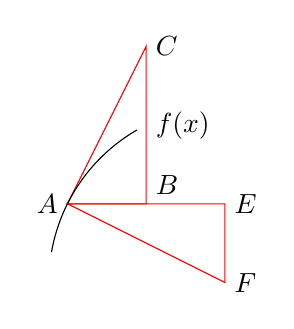
\begin{tikzpicture}
        \draw[color=red] (1,2) -- (2,2) -- (2,4) -- cycle;
        \draw[color=red] (1,2) -- (3,2) -- (3,1) -- cycle;
        \draw[color=black] (1,2) arc (153.43:120:2.24) node[pos=1.1,right]{$f(x)$};
        \draw[color=black] (1,2) arc (153.43:170:2.24);
        \node[left] (A) at (1,2) {$A$};
        \node[above right] (B) at (2,2) {$B$};
        \node[right] (C) at (2,4) {$C$};
        \node[right] (E) at (3,2) {$E$};
        \node[right] (F) at (3,1) {$F$};
    \end{tikzpicture}
\end{marginfigure}

\begin{proof}
    \begin{enumerate}[(1)]
        \item 一元函数$f(x)$的证明如下图,其中$AC$为切线,$|AB|=1$,则$|CB|=f'(x)$,那么得出向量
              $\overrightarrow{AC}=(1,f'(x))$,同时令$|EF|=1$根据$\triangle ABC \cong\triangle FEB$,
              那么$|AE|=f'(x)$,所以法向量$\overrightarrow{AF}=(f'(x),-1)$

        \item 设二元函数$z=f(x,y)$上的任意一点的法向量为$\bm{n}$,则$\bm{n}$在平面$xOz, yOz$的投影向量分别为,
              $(z_x',-1),(z_y',-1)$,因此$\bm{n} = (z_x',z_y',-1)$
    \end{enumerate}
\end{proof}

\subsection{二次曲面}
由三元二次方程所确定的曲面称为二次曲面。二次曲面与平面的交线都是二次曲线。

\subsubsection{椭球面}
由方程
\begin{equation}
    \frac{x^2}{a^2} + \frac{y^2}{b^2} + \frac{z^2}{c^2} = 1
\end{equation}
所确定的曲面称为椭球面。任意平面与椭球的交线均为椭圆。
\begin{marginfigure}
    \centering
    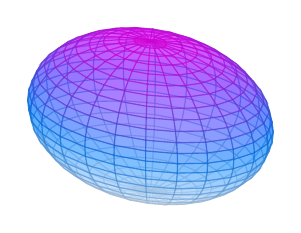
\begin{tikzpicture}
        \begin{axis}[hide axis,colormap/cool,z buffer=sort, opacity=0.5, axis equal]
            \addplot3[surf, domain=0:360,y domain=0:180] ({1.5*cos(x)*sin(y)},{sin(x)*sin(y)},{cos(y)});
        \end{axis}
    \end{tikzpicture}
    \caption{椭球面。}
\end{marginfigure}

\subsubsection{单叶双曲面}
分别由方程
\begin{align}
    \frac{x^2}{a^2} + \frac{y^2}{b^2} - \frac{z^2}{c^2}   & = 1 \\
    \frac{x^2}{a^2} - \frac{y^2}{b^2} + \frac{z^2}{c^2}   & = 1 \\
    - \frac{x^2}{a^2} + \frac{y^2}{b^2} + \frac{z^2}{c^2} & = 1
\end{align}
所确定的曲面称为单叶双曲面。
\begin{marginfigure}
    \centering
    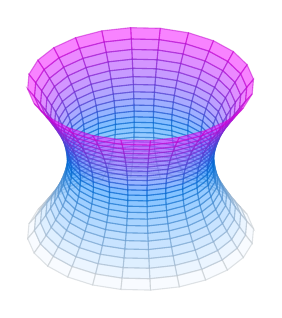
\begin{tikzpicture}
        \begin{axis}[hide axis,colormap/cool,z buffer=sort, opacity=0.5, axis equal]
            \addplot3[surf, domain=0:360,y domain=-1:1] ({cosh(y)*cos(x)},{cosh(y)*sin(x)},{sinh(y)});
        \end{axis}
    \end{tikzpicture}
    \caption{单叶双曲面。}
\end{marginfigure}

\subsubsection{二次锥面}
分别由方程
\begin{align}
    \frac{x^2}{a^2} + \frac{y^2}{b^2} - \frac{z^2}{c^2}   & = 0 \\
    \frac{x^2}{a^2} - \frac{y^2}{b^2} + \frac{z^2}{c^2}   & = 0 \\
    - \frac{x^2}{a^2} + \frac{y^2}{b^2} + \frac{z^2}{c^2} & = 0
\end{align}
所确定的曲面称为二次锥面。
\begin{marginfigure}
    \centering
    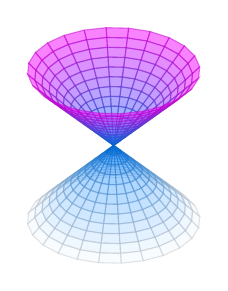
\begin{tikzpicture}
        \begin{axis}[hide axis,colormap/cool,z buffer=sort, opacity=0.5, axis equal]
            \addplot3[surf, domain=0:360,y domain=-1:1] ({y*cos(x)},{y*sin(x)},{y});
        \end{axis}
    \end{tikzpicture}
    \caption{二次锥面。}
\end{marginfigure}

\subsubsection{双叶双曲线}
分别由方程$(pq>0)$
\begin{align}
    \frac{x^2}{a^2} + \frac{y^2}{b^2} - \frac{z^2}{c^2}   & = -1 \\
    \frac{x^2}{a^2} - \frac{y^2}{b^2} + \frac{z^2}{c^2}   & = -1 \\
    - \frac{x^2}{a^2} + \frac{y^2}{b^2} + \frac{z^2}{c^2} & = -1
\end{align}
所确定的曲面称为双叶双曲线。
\begin{marginfigure}
    \centering
    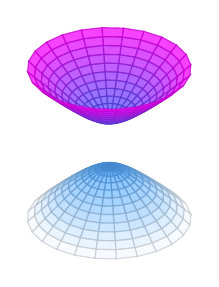
\begin{tikzpicture}
        \begin{axis}[hide axis,colormap/cool,z buffer=sort, opacity=0.5, axis equal]
            \addplot3[surf, domain=0:360,y domain=-3:3] ({y*cos(x)},{y*sin(x)},{sqrt(y^2+1)});
            \addplot3[surf, domain=0:360,y domain=-3:3] ({y*cos(x)},{y*sin(x)},{-sqrt(y^2+1)});
        \end{axis}
    \end{tikzpicture}
    \caption{双叶双曲线。}
\end{marginfigure}

\subsubsection{双曲抛物面}
分别由方程
\begin{align}
    z = -\frac{x^2}{2p} + \frac{y^2}{2q} \\
    x = -\frac{y^2}{2p} + \frac{z^2}{2q} \\
    y = -\frac{z^2}{2p} + \frac{x^2}{2q}
\end{align}
所确定的曲面称为双曲抛物面。
\begin{marginfigure}
    \centering
    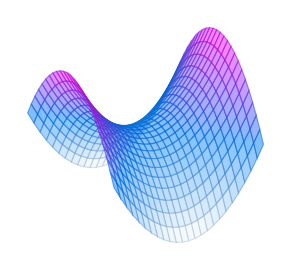
\begin{tikzpicture}
        \begin{axis}[hide axis,colormap/cool,z buffer=sort, opacity=0.5, axis equal,view/h=60]
            \addplot3[surf] {0.2*(-x^2+y^2)};
        \end{axis}
    \end{tikzpicture}
    \caption{双曲抛物面。}
\end{marginfigure}

\subsubsection{椭圆抛物面}
分别由方程
\begin{align}
    z = \frac{x^2}{2p} + \frac{y^2}{2q} \\
    x = \frac{y^2}{2p} + \frac{z^2}{2q} \\
    y = \frac{z^2}{2p} + \frac{x^2}{2q}
\end{align}
所确定的曲面称为椭圆抛物面。
\begin{marginfigure}
    \centering
    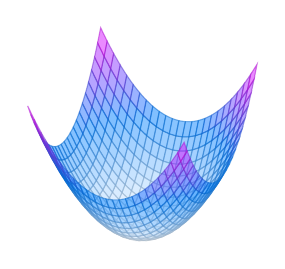
\begin{tikzpicture}
        \begin{axis}[hide axis,colormap/cool,z buffer=sort, opacity=0.5, axis equal]
            \addplot3[surf] {0.2*(x^2+y^2)};
        \end{axis}
    \end{tikzpicture}
    \caption{椭圆抛物面。}
\end{marginfigure}

对于截面曲线的判断,只需要让其中一个分量等于零,在根据平面曲线来判断曲线的 类型。